\documentclass[10pt,twocolumn]{article}
\usepackage[margin=0.67in,columnsep=0.24in]{geometry}
\usepackage{amsmath,amssymb,booktabs,graphicx,microtype}
\usepackage{enumitem}
\usepackage{xcolor}
\usepackage[hidelinks]{hyperref}
\usepackage{siunitx}
\usepackage{url}

\newcommand{\method}{DualDeadline}
\newcommand{\ms}{\,\mathrm{ms}}
\setlist{nosep,leftmargin=*}
\setlength{\textfloatsep}{7pt plus 2pt minus 2pt}
\setlength{\floatsep}{6pt plus 2pt minus 2pt}
\setlength{\intextsep}{6pt plus 2pt minus 2pt}

\title{\vspace{-1.5em}\method: Component-Staged Expert Prefetching\\
for Exact Offloaded Mixture-of-Experts Inference}
\author{Anonymous Authors}
\date{}

\begin{document}
\maketitle
\vspace{-1.4em}

\begin{abstract}
Expert prefetch predictors usually treat an expert as an indivisible transfer.
We ask whether the structure already present inside a gated mixture-of-experts
(MoE) feed-forward block creates a second, useful transfer deadline.
\method{} predicts only the gate and up projections before the authoritative
router fires.  Once the native top-$k$ route is known, it transfers the down
projections while gate/up computation executes.  Prediction remains advisory:
misses are loaded on demand and the frozen router and expert arithmetic are
unchanged.

We evaluate this post-hoc design on OLMoE-1B-7B-Instruct using autoregressive
router traces and pinned-host-memory measurements from one PCIe-attached
NVIDIA H200.  A preregistered 120-prompt pilot reaches 45.23\% held-out
expert recall with four candidates, versus 26.74\% for training-set
popularity; a prompt-disjoint 300-prompt replication reaches 46.63\%.
At an equal four-expert byte budget, trace replay estimates
$1.223\ms$ exposed stall for monolithic prefetch and $1.106\ms$ for
component staging.  A real CUDA-stream microbenchmark with eight OLMoE
experts reduces block latency from $2.193\ms$ to $1.939\ms$ without numerical
change.  Benefits persist under prompt-cold LRU caches from 8 to 64 experts
per layer.  We distinguish measured microbenchmarks from trace-driven
simulation and do not claim end-to-end serving speedup.
\end{abstract}

\section{Introduction}
Sparse MoE models increase total capacity while activating only a few experts
per token \cite{shazeer2017moe,fedus2022switch}.  When the expert pool does
not fit accelerator memory, inactive weights can remain in host memory and be
copied on demand.  The native route, however, is available only after the
router executes, placing host-to-device transfer on the decode critical path.

SpecPrefetch \cite{kong2026specprefetch} introduced a clean transfer-only
design: a small post-hoc adapter predicts next-layer experts early, but the
native router still controls execution.  False predictions therefore waste
bandwidth rather than change logits.  Its scheduler reasons about whether a
whole predicted expert can arrive before execution.  We investigate an
orthogonal question: \emph{must the entire expert share one deadline?}

A gated expert naturally contains three matrices:
\begin{equation}
y_e = W^{e}_{d}\left[
  \operatorname{SiLU}(W^{e}_{g}x)\odot W^{e}_{u}x
\right].
\label{eq:expert}
\end{equation}
For OLMoE, $W_g$ and $W_u$ together occupy two thirds of the expert bytes;
$W_d$ occupies one third.  The down matrix is not consumed until after
gate/up arithmetic has produced the intermediate activation.  This dependency
creates a second transfer-compute overlap opportunity.

Our contributions are:
\begin{itemize}
  \item a router-preserving, component-staged schedule that speculates on
  gate/up weights and transfers authoritative down weights during compute;
  \item deadline-aware evaluation that charges predictor latency and uses
  measured transfer and layer windows instead of recall alone;
  \item a preregistered held-out study, a prompt-disjoint replication, cache
  sensitivity, and a real-stream overlap microbenchmark on an H200; and
  \item bounded forward-pass optimization experiments, including algebraic
  low-rank materialization, CUDA Graphs, \texttt{torch.compile}, and custom
  Triton kernels, with both positive and negative results reported.
\end{itemize}

\section{Background and Related Work}
\paragraph{Router-preserving prefetch.}
SpecPrefetch predicts the expert set at layer $l+1$ from router input at layer
$l$, then schedules only transfers that can finish within the measured window
\cite{kong2026specprefetch}.  FATE instead exploits adjacent-layer gate
regularity without learned parameters \cite{fang2025fate}.  ExpertFlow adapts
prediction horizon to runtime conditions \cite{shen2025expertflow}, while
OD-MoE predicts multiple layers ahead in a distributed cacheless setting
\cite{wang2025odmoe}.  We retain the next-layer, transfer-only contract and
change expert transfer granularity.

\paragraph{Earlier same-layer information and finer caching.}
Pre-attention prediction learns same-layer routes from the state before
attention \cite{zhu2025preattention}; we include this as an exploratory horizon
control rather than a novelty claim.  SliceMoE caches bit slices at different
precision \cite{choi2025slicemoe}.  Our components follow the exact
computational dependency in Eq.~\ref{eq:expert}; no quantization or approximate
execution is introduced.

\section{\method{}}
\subsection{Transfer-only prediction}
Let $\mathcal{T}^{l+1}$ be the native top-$k$ expert set and
$s^{l+1}\in\mathbb{R}^{E}$ be advisory scores predicted from layer-$l$ router
input.  The executed set remains $\mathcal{T}^{l+1}$ for every policy.  A
missing component is synchronously copied before use, hence prediction errors
cannot change the mathematical forward pass.

Our primary predictor is shared across layers.  It applies layer normalization,
a width-256 hidden projection, a 32-dimensional target-layer embedding
projected to width 256, GELU, and a 64-way output.  It has 553,536 trainable
parameters; the base model is frozen.  Multi-label binary cross entropy uses
the native top-8 route as target.  Checkpoint selection maximizes validation
ready recall after measured predictor and transfer deadlines.

\subsection{Two component deadlines}
Before the target router, the scheduler copies predicted $(W_g,W_u)$ pairs in
score order.  Let $G$ be those ready pairs and let $\mathcal{T}$ be the native
route revealed at the target router.  Experts in $G\cap\mathcal{T}$ can start
gate/up compute immediately.  Down matrices are never selected by the
speculative predictor: after routing, the scheduler copies
$\{W_d^e:e\in\mathcal{T}\}$ on a DMA stream while gate/up kernels execute on a
compute stream.  Gate/up misses are copied on demand.  With one DMA channel,
our conservative replay model is
\begin{equation}
S_{\mathrm{stage}} =
(k-|G\cap\mathcal{T}|)\,t_{gu}
+ \max(0, k\,t_d-t_{\mathrm{compute},gu}),
\label{eq:stall}
\end{equation}
before persistent-cache hits are removed.  The monolithic comparison charges
$(k-|F\cap\mathcal{T}|)t_{\mathrm{full}}$ for ready full experts $F$.  Both
receive the same speculative byte budget.

\subsection{Runtime and cache model}
We subtract batch-1 predictor latency from the measured issue-to-router
window.  Transfers are feasible only if their estimated completion precedes
the target router.  Cache replay uses an independent full-expert LRU per layer,
reset at each prompt.  Speculative components use a separate bounded workspace
and unused predictions are discarded at the target layer.  This isolates
prefetch value from cache pollution; alternative shared-pool policies remain
future work.

\section{Experimental Method}
\paragraph{Model and hardware.}
OLMoE-1B-7B-Instruct has 7B total and about 1B active parameters
\cite{muennighoff2024olmoe}.  It contains 16 MoE layers, 64 experts per layer,
and activates 8 experts per token.  Experiments use bfloat16 on one NVIDIA H200
with 141\,GB HBM attached over PCIe Gen5 x16.  We pin host tensors and use
PyTorch 2.9.1, CUDA 12.8, Transformers 5.14.1, and Triton 3.5.1.

\paragraph{Data and traces.}
The preregistered pilot contains 80 GSM8K and 40 HumanEval prompts, split
60/20/20 by prompt.  Greedy autoregressive decoding produces 10,872 decode
steps; the 24-prompt test set contains 32,520 target layer-token pairs.
After the pilot result, we add a clearly labeled exploratory replication with
200 GSM8K and 100 HumanEval prompts whose IDs are disjoint from the pilot.
Its 60-prompt test set contains 81,195 pairs.  Native routes, full router logits,
router inputs, and layer-start states are detached and stored; prompts, never
tokens, are the split and bootstrap unit.

\paragraph{Policies and statistics.}
We compare random scores, training-set popularity, previous-layer native
routes (training-free), learned prediction, and an oracle.  Reported intervals
are paired 2,000-resample percentile bootstraps over prompts.  The simulator
uses measured p50 layer windows and a linear fit to pinned host-to-device
copies.  Results explicitly labeled ``simulation'' are not end-to-end serving
measurements.

\section{Results}
\subsection{Held-out expert prediction}
\begin{table}[t]
\centering
\small
\caption{Pilot held-out expert recall (\%).  ``Rep.'' is the disjoint
replication for the primary learned predictor.}
\label{tab:recall}
\begin{tabular}{lrrr}
\toprule
Policy & R@2 & R@4 & R@8\\
\midrule
Random & 3.16 & 6.24 & 12.41\\
Previous-layer route & 3.09 & 6.09 & 12.24\\
Training popularity & 16.34 & 26.74 & 41.15\\
Learned (primary) & \textbf{23.69} & \textbf{45.23} & \textbf{76.33}\\
Oracle & 25.00 & 50.00 & 100.00\\
\midrule
Learned (Rep.) & 24.15 & 46.63 & 79.77\\
\bottomrule
\end{tabular}
\end{table}

Table~\ref{tab:recall} shows that hidden-state prediction captures information
not present in previous expert IDs alone.  At budget four, learned-minus-
popularity is +18.49 percentage points in the pilot (95\% CI
[+17.68,+19.27]) and +20.45 points in the replication
([+19.82,+21.04]).  Pilot R@4 is 44.43\% on GSM8K and 45.15\% on HumanEval for
the earlier direct-embedding control; the primary conformant checkpoint shows
the same qualitative task stability.

\begin{figure}[t]
\centering
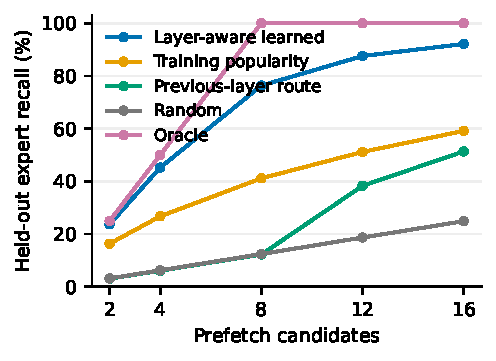
\includegraphics[width=\columnwidth]{figures/predictor_recall.pdf}
\caption{Held-out pilot recall under a fixed candidate budget.}
\label{fig:recall}
\end{figure}

\subsection{Measured component overlap}
Pinned-copy p50 times are 0.159\,ms for an 8\,MiB gate/up component,
0.083\,ms for a 4\,MiB down component, and 0.234\,ms for a 12\,MiB full
expert.  Eight experts' gate/up and down arithmetic take 0.257\,ms and
0.128\,ms, respectively.  The next-layer issue-to-router window is
0.81--0.89\,ms before predictor cost; the primary predictor costs 0.102\,ms
including the bfloat16-to-float32 input cast.  Thus four gate/up transfers are
feasible on all 15 target layers.

\begin{figure}[t]
\centering
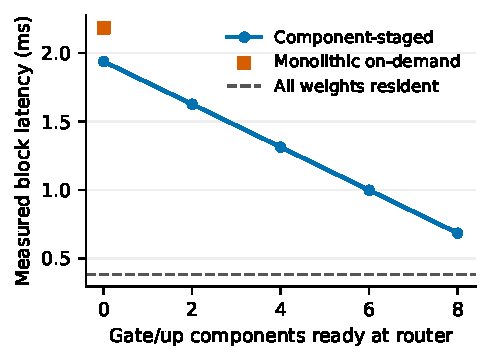
\includegraphics[width=\columnwidth]{figures/measured_overlap.pdf}
\caption{Real pinned-memory copies and CUDA streams using eight layer-0 OLMoE
experts.  Outputs match resident execution exactly.}
\label{fig:overlap}
\end{figure}

With real tensors, resident compute takes 0.382\,ms, monolithic copy then
compute takes 2.185\,ms, and serial component reordering takes 2.194\,ms.
Actual two-stream staging takes 1.938\,ms.  Therefore concurrency, not
reordering, saves 0.247\,ms in this run.  Making 2, 4, 6, and 8 gate/up
components ready before the router reduces latency monotonically to
1.626, 1.312, 0.998, and 0.683\,ms.  All strategies are numerically identical
to resident execution.  Repeating the full-transfer comparison independently
on all 16 layers gives a median 2.192\,ms for monolithic loading and
1.938\,ms for staging, a median saving of 0.254\,ms (11.6\%); the
layerwise saving ranges from 0.247 to 0.390\,ms, with zero numerical error.
Nine independent repeats on layers 0, 7, and 15 give a 0.253\,ms mean saving
with 0.0049\,ms sample standard deviation.  At layer 0, varying routed top-$k$
from 1, 2, 4, to 8 gives absolute savings of 0.063, 0.061, 0.122, and
0.254\,ms.

\subsection{Trace-driven stall and cache sensitivity}
\begin{figure}[t]
\centering
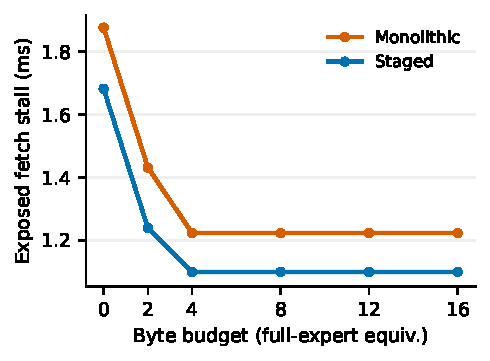
\includegraphics[width=\columnwidth]{figures/cacheless_stall.pdf}
\caption{Cacheless pilot replay for the primary learned predictor.  Bands are
95\% prompt-bootstrap intervals and are often narrower than the line.}
\label{fig:stall}
\end{figure}

At four full-expert byte equivalents, monolithic replay exposes
1.223\,ms per layer-token and staging exposes 1.106\,ms; the paired difference
is -0.117\,ms (95\% CI [-0.118,-0.115]).  The disjoint replication gives
1.207\,ms and 1.089\,ms, a -0.118\,ms difference
([-0.1187,-0.1176]).  Larger byte budgets do not help because the measured
deadline, rather than capacity, is binding.  Replacing the mean-copy fit with
a p95-copy fit increases the staging advantage to -0.225\,ms.

\begin{figure}[t]
\centering
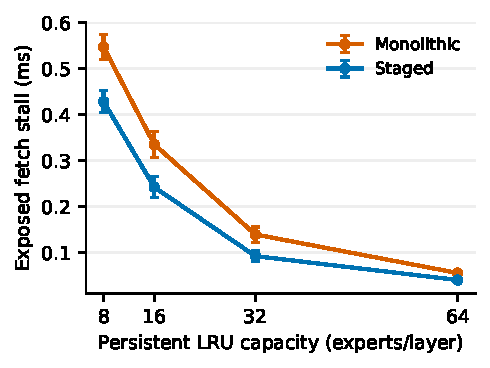
\includegraphics[width=\columnwidth]{figures/cache_sensitivity.pdf}
\caption{Prompt-cold per-layer LRU sensitivity at byte budget four.}
\label{fig:cache}
\end{figure}

The primary conformant checkpoint shows that staged benefit persists from 8
to 64 cached experts per layer: at capacity 8, exposed stall is 0.547\,ms
monolithic and 0.432\,ms staged; at capacity 64 it is 0.055\,ms and
0.040\,ms.  Intermediate capacities 16 and 32 give
0.335/0.245\,ms and 0.139/0.093\,ms, respectively.

\subsection{Predictor and forward-pass ablations}
\begin{table}[t]
\centering
\footnotesize
\setlength{\tabcolsep}{4pt}
\caption{Exploratory predictor controls on the pilot.}
\label{tab:ablations}
\begin{tabular}{lrr}
\toprule
Predictor & Parameters & R@4 (\%)\\
\midrule
Layer-aware, width 64 & 140,352 & 39.02\\
Layer-aware, width 128 & 276,544 & 42.41\\
Layer-aware, width 256 direct emb. & 548,928 & 44.67\\
Layer-aware, width 256, emb. 32 & 553,536 & \textbf{45.23}\\
Shared low-rank, KL & 540,672 & 34.67\\
Shared low-rank, BCE & 540,672 & 35.53\\
\bottomrule
\end{tabular}
\end{table}

Deadline-weighted BCE is effectively tied with and slightly below uniform BCE
(44.65\% versus 44.67\% R@4 in the direct-embedding control), so we retain the
simpler loss.  Across the primary conformant checkpoint and two additional
training seeds, pilot R@4 is 45.20\% with a 0.03-point sample standard
deviation; the corresponding disjoint-replication result is 46.60\% with a
0.03-point standard deviation.

For the linear low-rank control, the two matrices can be multiplied once after
training.  This exact materialization reduces batch-1 p50 from 0.0388\,ms to
0.0212\,ms.  A tuned custom Triton GEMV reaches 0.0273\,ms and is faster than
the factorized adapter but slower than PyTorch's materialized GEMV; maximum
error is below $3\times10^{-7}$.  On the conformant layer-aware model,
\emph{post-training} layer-table materialization cuts the matched eager path
from 0.1013 to 0.0840\,ms; a custom two-kernel Triton path reaches
0.0635\,ms, 35.8\% below its 0.0989-ms eager baseline.  Top-2/4/8 sets agree
on all 32,520 pilot and 81,195 replication pairs (maximum differences
$5.7\times10^{-6}$ and $6.7\times10^{-6}$).  Qwen-shaped materialization
cuts 0.1016 to 0.0830\,ms.
\texttt{torch.compile} is slower with already-float32 input
(0.140\,ms versus 0.092\,ms eager).  In contrast, a static CUDA Graph costs
0.0225\,ms to replay and 0.0326\,ms including the bfloat16 input conversion,
versus 0.1065\,ms for the matched eager path, with identical output.  The
primary deadline analysis conservatively retains the measured non-graph eager
cost.  These results argue for measuring small-kernel launch behavior rather
than assuming a compiler or custom kernel must win
\cite{tillet2019triton}.

\section{Limitations}
Our end-to-end claims are deliberately narrow.  Trace replay assumes one DMA
channel and measured p50 windows; only expert-block overlap uses real streams.
We do not integrate with a production scheduler or measure cross-request PCIe
contention or batched throughput.  The simulator gives speculative weights a
separate workspace and resets LRU per prompt.  OLMoE is smaller than frontier
MoEs, so results must not be extrapolated to trillion-parameter models without
measurement.  The replication, low-rank control, and systems ablations are
post-pilot and labeled exploratory in the machine-readable protocol.

\section{Conclusion}
An expert need not have one transfer deadline.  Moving gate/up weights first
and authoritative down weights during gate/up computation preserves exact
routing while reducing speculative bytes and exposed stall.  On OLMoE and an
H200, the effect survives held-out prompts, a larger disjoint replication,
cache sensitivity, and direct CUDA-stream measurement.  The study also shows
why ready recall, predictor latency, and real overlap must be reported
together.  A production offloading integration and validation on larger MoEs
are the necessary next steps.

\bibliographystyle{unsrt}
\bibliography{references}

\end{document}
